\documentclass[tikz,border=3pt]{standalone}
\usepackage{times}
\usepackage{amsmath,amssymb}
\usepackage{siunitx}
\usepackage{graphicx}
\usepackage{pgfplots}
\pgfplotsset{compat=1.18}
\usepgfplotslibrary{groupplots,fillbetween,colorbrewer}
\usetikzlibrary{arrows.meta,positioning,calc,fit,backgrounds,shapes.geometric,decorations.pathreplacing,patterns,matrix}
\graphicspath{{../}{../figures/}}
\definecolor{cmpc}{HTML}{C0392B}
\definecolor{csch}{HTML}{1F5FA8}
\definecolor{cstk}{HTML}{6E6E6E}
\definecolor{cband}{HTML}{F4C7C3}
\definecolor{crec}{HTML}{2B2B2B}
\definecolor{cphase}{HTML}{FBE3C2}
\newlength{\pw}\newlength{\ph}
\pgfplotsset{
  paperaxis/.style={scale only axis, tick label style={font=\scriptsize}, label style={font=\footnotesize}, title style={font=\footnotesize, yshift=-1mm},
    legend style={font=\scriptsize, draw=black!25, fill=white, legend cell align=left, /tikz/every even column/.append style={column sep=6pt}}, axis line style={black!60}, tick style={black!60}, every axis plot/.append style={line width=0.9pt},
    grid=major, grid style={black!12}, xlabel near ticks, ylabel near ticks, ylabel shift=-2pt, xlabel shift=-2pt, clip marker paths=true},
}
\newcommand{\panel}[2]{\node[anchor=north west, font=\footnotesize\bfseries, inner sep=1.5pt, fill=white, fill opacity=0.85, text opacity=1] at (rel axis cs:0.015,0.985) {(#1)#2};}
\newcommand{\gth}{g_\theta}
\newcommand{\thsp}{\theta_{\mathrm{sp}}}

\pgfplotsset{discard if not/.style 2 args={x filter/.append code={\edef\tempa{\thisrow{#1}}\edef\tempb{#2}\ifx\tempa\tempb\else\def\pgfmathresult{inf}\fi}}}

\definecolor{mDR}{HTML}{E4EEF9}\definecolor{mRO}{HTML}{FFF1E0}\definecolor{mLS}{HTML}{E6F4E1}
\definecolor{bLin}{HTML}{4A78B5}\definecolor{bQP}{HTML}{C0392B}\definecolor{bAtt}{HTML}{E08A2E}
\tikzset{mod/.style={draw=black!40, rounded corners=5pt, fill=#1, inner sep=0pt}, modtitle/.style={font=\footnotesize\bfseries, anchor=north west, inner sep=4pt},
  blk/.style={draw=#1, fill=#1!15, rounded corners=2pt, font=\scriptsize, minimum height=5.2mm, inner sep=3pt, align=center},
  arr/.style={-{Latex[length=1.8mm]}, line width=0.6pt, black!70}, farr/.style={-{Latex[length=2.4mm]}, line width=1.1pt, black!80},
  note/.style={font=\scriptsize, align=left, inner sep=1pt}}
\begin{document}
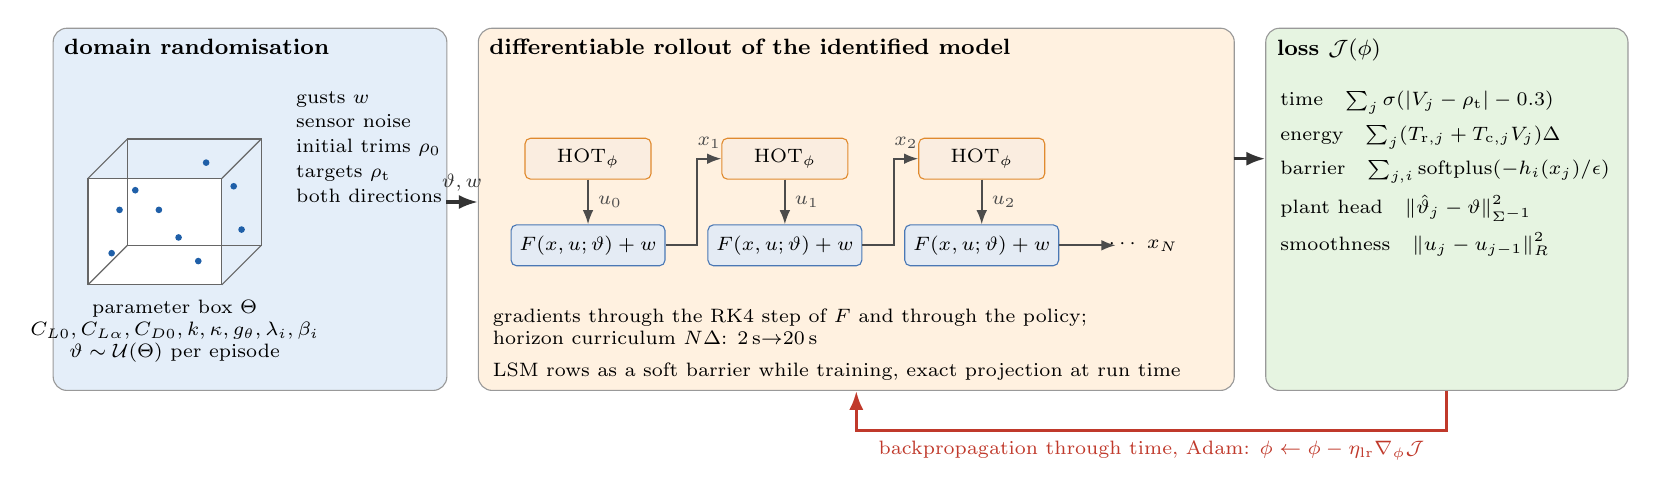
\begin{tikzpicture}[x=1cm,y=1cm]
% ---- domain randomisation ----
\node[mod=mDR, minimum width=5.0cm, minimum height=4.6cm, anchor=south west] (dr) at (0,0) {};
\node[modtitle] at (dr.north west) {domain randomisation};
\begin{scope}[shift={(0.45,1.35)}]
\draw[black!60, fill=white] (0,0) rectangle (1.7,1.35); \draw[black!60] (0.5,0.5) rectangle (2.2,1.85); \draw[black!60] (0,1.35)--(0.5,1.85) (1.7,1.35)--(2.2,1.85) (1.7,0)--(2.2,0.5) (0,0)--(0.5,0.5);
\foreach \p in {(0.3,0.4),(0.9,0.95),(1.4,0.3),(0.6,1.2),(1.85,1.25),(1.15,0.6),(1.95,0.7),(0.4,0.95),(1.5,1.55)} \fill[csch] \p circle (1.2pt);
\end{scope}
\node[note, anchor=north, align=center] at (1.55,1.2) {parameter box $\Theta$\\ $C_{L0},C_{L\alpha},C_{D0},k,\kappa,\gth,\lambda_i,\beta_i$\\ $\vartheta\sim\mathcal U(\Theta)$ per episode};
\node[note, anchor=north west] at (3.05,3.85) {gusts $w$\\[1pt] sensor noise\\[1pt] initial trims $\rho_0$\\[1pt] targets $\rho_{\mathrm t}$\\[1pt] both directions};
% ---- differentiable rollout ----
\node[mod=mRO, minimum width=9.6cm, minimum height=4.6cm, anchor=south west] (ro) at (5.4,0) {};
\node[modtitle] at (ro.north west) {differentiable rollout of the identified model};
\foreach \i/\x in {0/6.1,1/8.6,2/11.1}{
  \node[blk=bAtt, minimum width=16mm] (h\i) at (\x+0.7,2.95) {HOT$_\phi$};
  \node[blk=bLin, minimum width=16mm] (f\i) at (\x+0.7,1.85) {$F(x,u;\vartheta)+w$};
  \draw[arr] (h\i) -- node[right, font=\scriptsize] {$u_{\i}$} (f\i);}
\node[font=\scriptsize] at (13.85,1.85) {$\cdots\ x_N$};
\draw[arr] (f0.east) -- ++(0.4,0) |- node[pos=0.75, above, font=\scriptsize] {$x_1$} (h1.west);
\draw[arr] (f1.east) -- ++(0.4,0) |- node[pos=0.75, above, font=\scriptsize] {$x_2$} (h2.west);
\draw[arr] (f2.east) -- (13.5,1.85);
\draw[farr] (5.0,2.4) -- node[above, font=\scriptsize] {$\vartheta,w$} (5.4,2.4);
\node[note, anchor=south west] at (5.55,0.55) {gradients through the RK4 step of $F$ and through the policy;\\ horizon curriculum $N\Delta$: \SI{2}{s}$\to$\SI{20}{s}};
\node[note, anchor=south west] at (5.55,0.1) {LSM rows as a soft barrier while training, exact projection at run time};
% ---- losses ----
\node[mod=mLS, minimum width=4.6cm, minimum height=4.6cm, anchor=south west] (ls) at (15.4,0) {};
\node[modtitle] at (ls.north west) {loss $\mathcal J(\phi)$};
\node[note, anchor=north west] at (15.55,3.85) {time\quad $\sum_j\sigma(|V_j-\rho_{\mathrm t}|-0.3)$\\[3pt] energy\quad $\sum_j(T_{\mathrm r,j}+T_{\mathrm c,j}V_j)\Delta$\\[3pt] barrier\quad $\sum_{j,i}\mathrm{softplus}(-h_i(x_j)/\epsilon)$\\[3pt] plant head\quad $\|\hat\vartheta_j-\vartheta\|^2_{\Sigma^{-1}}$\\[3pt] smoothness\quad $\|u_j-u_{j-1}\|^2_R$};
\draw[farr] (15.0,2.95) -- (15.4,2.95);
% ---- BPTT ----
\draw[farr, bQP] (ls.south) -- ++(0,-0.5) -| node[pos=0.25, below, font=\scriptsize, bQP] {backpropagation through time, Adam: $\phi\leftarrow\phi-\eta_{\mathrm{lr}}\nabla_\phi\mathcal J$} (ro.south);
\end{tikzpicture}
\end{document}
